\documentclass{ximera}

%\usepackage{todonotes}

\newcommand{\todo}{}

\usepackage{esint} % for \oiint
\ifxake%%https://math.meta.stackexchange.com/questions/9973/how-do-you-render-a-closed-surface-double-integral
\renewcommand{\oiint}{{\large\bigcirc}\kern-1.56em\iint}
\fi


\graphicspath{
  {./}
  {ximeraTutorial/}
  {basicPhilosophy/}
  {functionsOfSeveralVariables/}
  {normalVectors/}
  {lagrangeMultipliers/}
  {vectorFields/}
  {greensTheorem/}
  {shapeOfThingsToCome/}
  {dotProducts/}
  {partialDerivativesAndTheGradientVector/}
  {../productAndQuotientRules/exercises/}
  {../normalVectors/exercisesParametricPlots/}
  {../continuityOfFunctionsOfSeveralVariables/exercises/}
  {../partialDerivativesAndTheGradientVector/exercises/}
  {../directionalDerivativeAndChainRule/exercises/}
  {../commonCoordinates/exercisesCylindricalCoordinates/}
  {../commonCoordinates/exercisesSphericalCoordinates/}
  {../greensTheorem/exercisesCurlAndLineIntegrals/}
  {../greensTheorem/exercisesDivergenceAndLineIntegrals/}
  {../shapeOfThingsToCome/exercisesDivergenceTheorem/}
  {../greensTheorem/}
  {../shapeOfThingsToCome/}
  {../separableDifferentialEquations/exercises/}
  {vectorFields/}
}

\newcommand{\mooculus}{\textsf{\textbf{MOOC}\textnormal{\textsf{ULUS}}}}

\usepackage{tkz-euclide}
\usepackage{tikz}
\usepackage{tikz-cd}
\usetikzlibrary{arrows}
\tikzset{>=stealth,commutative diagrams/.cd,
  arrow style=tikz,diagrams={>=stealth}} %% cool arrow head
\tikzset{shorten <>/.style={ shorten >=#1, shorten <=#1 } } %% allows shorter vectors

\usetikzlibrary{backgrounds} %% for boxes around graphs
\usetikzlibrary{shapes,positioning}  %% Clouds and stars
\usetikzlibrary{matrix} %% for matrix
\usepgfplotslibrary{polar} %% for polar plots
\usepgfplotslibrary{fillbetween} %% to shade area between curves in TikZ
%\usetkzobj{all}
\usepackage[makeroom]{cancel} %% for strike outs
%\usepackage{mathtools} %% for pretty underbrace % Breaks Ximera
%\usepackage{multicol}
\usepackage{pgffor} %% required for integral for loops



%% http://tex.stackexchange.com/questions/66490/drawing-a-tikz-arc-specifying-the-center
%% Draws beach ball
\tikzset{pics/carc/.style args={#1:#2:#3}{code={\draw[pic actions] (#1:#3) arc(#1:#2:#3);}}}



\usepackage{array}
\setlength{\extrarowheight}{+.1cm}
\newdimen\digitwidth
\settowidth\digitwidth{9}
\def\divrule#1#2{
\noalign{\moveright#1\digitwidth
\vbox{\hrule width#2\digitwidth}}}




% \newcommand{\RR}{\mathbb R}
% \newcommand{\R}{\mathbb R}
% \newcommand{\N}{\mathbb N}
% \newcommand{\Z}{\mathbb Z}

\newcommand{\sagemath}{\textsf{SageMath}}


%\renewcommand{\d}{\,d\!}
%\renewcommand{\d}{\mathop{}\!d}
%\newcommand{\dd}[2][]{\frac{\d #1}{\d #2}}
%\newcommand{\pp}[2][]{\frac{\partial #1}{\partial #2}}
% \renewcommand{\l}{\ell}
%\newcommand{\ddx}{\frac{d}{\d x}}

% \newcommand{\zeroOverZero}{\ensuremath{\boldsymbol{\tfrac{0}{0}}}}
%\newcommand{\inftyOverInfty}{\ensuremath{\boldsymbol{\tfrac{\infty}{\infty}}}}
%\newcommand{\zeroOverInfty}{\ensuremath{\boldsymbol{\tfrac{0}{\infty}}}}
%\newcommand{\zeroTimesInfty}{\ensuremath{\small\boldsymbol{0\cdot \infty}}}
%\newcommand{\inftyMinusInfty}{\ensuremath{\small\boldsymbol{\infty - \infty}}}
%\newcommand{\oneToInfty}{\ensuremath{\boldsymbol{1^\infty}}}
%\newcommand{\zeroToZero}{\ensuremath{\boldsymbol{0^0}}}
%\newcommand{\inftyToZero}{\ensuremath{\boldsymbol{\infty^0}}}



% \newcommand{\numOverZero}{\ensuremath{\boldsymbol{\tfrac{\#}{0}}}}
% \newcommand{\dfn}{\textbf}
% \newcommand{\unit}{\,\mathrm}
% \newcommand{\unit}{\mathop{}\!\mathrm}
% \newcommand{\eval}[1]{\bigg[ #1 \bigg]}
% \newcommand{\seq}[1]{\left( #1 \right)}
% \renewcommand{\epsilon}{\varepsilon}
% \renewcommand{\phi}{\varphi}


% \renewcommand{\iff}{\Leftrightarrow}

% \DeclareMathOperator{\arccot}{arccot}
% \DeclareMathOperator{\arcsec}{arcsec}
% \DeclareMathOperator{\arccsc}{arccsc}
% \DeclareMathOperator{\si}{Si}
% \DeclareMathOperator{\scal}{scal}
% \DeclareMathOperator{\sign}{sign}


%% \newcommand{\tightoverset}[2]{% for arrow vec
%%   \mathop{#2}\limits^{\vbox to -.5ex{\kern-0.75ex\hbox{$#1$}\vss}}}
% \newcommand{\arrowvec}[1]{{\overset{\rightharpoonup}{#1}}}
% \renewcommand{\vec}[1]{\arrowvec{\mathbf{#1}}}
% \renewcommand{\vec}[1]{{\overset{\boldsymbol{\rightharpoonup}}{\mathbf{#1}}}}

% \newcommand{\point}[1]{\left(#1\right)} %this allows \vector{ to be changed to \vector{ with a quick find and replace
% \newcommand{\pt}[1]{\mathbf{#1}} %this allows \vec{ to be changed to \vec{ with a quick find and replace
% \newcommand{\Lim}[2]{\lim_{\point{#1} \to \point{#2}}} %Bart, I changed this to point since I want to use it.  It runs through both of the exercise and exerciseE files in limits section, which is why it was in each document to start with.

% \DeclareMathOperator{\proj}{\mathbf{proj}}
% \newcommand{\veci}{{\boldsymbol{\hat{\imath}}}}
% \newcommand{\vecj}{{\boldsymbol{\hat{\jmath}}}}
% \newcommand{\veck}{{\boldsymbol{\hat{k}}}}
% \newcommand{\vecl}{\vec{\boldsymbol{\l}}}
% \newcommand{\uvec}[1]{\mathbf{\hat{#1}}}
% \newcommand{\utan}{\mathbf{\hat{t}}}
% \newcommand{\unormal}{\mathbf{\hat{n}}}
% \newcommand{\ubinormal}{\mathbf{\hat{b}}}

% \newcommand{\dotp}{\bullet}
% \newcommand{\cross}{\boldsymbol\times}
% \newcommand{\grad}{\boldsymbol\nabla}
% \newcommand{\divergence}{\grad\dotp}
% \newcommand{\curl}{\grad\cross}
%\DeclareMathOperator{\divergence}{divergence}
%\DeclareMathOperator{\curl}[1]{\grad\cross #1}
% \newcommand{\lto}{\mathop{\longrightarrow\,}\limits}

% \renewcommand{\bar}{\overline}

\colorlet{textColor}{black}
\colorlet{background}{white}
\colorlet{penColor}{blue!50!black} % Color of a curve in a plot
\colorlet{penColor2}{red!50!black}% Color of a curve in a plot
\colorlet{penColor3}{red!50!blue} % Color of a curve in a plot
\colorlet{penColor4}{green!50!black} % Color of a curve in a plot
\colorlet{penColor5}{orange!80!black} % Color of a curve in a plot
\colorlet{penColor6}{yellow!70!black} % Color of a curve in a plot
\colorlet{fill1}{penColor!20} % Color of fill in a plot
\colorlet{fill2}{penColor2!20} % Color of fill in a plot
\colorlet{fillp}{fill1} % Color of positive area
\colorlet{filln}{penColor2!20} % Color of negative area
\colorlet{fill3}{penColor3!20} % Fill
\colorlet{fill4}{penColor4!20} % Fill
\colorlet{fill5}{penColor5!20} % Fill
\colorlet{gridColor}{gray!50} % Color of grid in a plot

\newcommand{\surfaceColor}{violet}
\newcommand{\surfaceColorTwo}{redyellow}
\newcommand{\sliceColor}{greenyellow}




\pgfmathdeclarefunction{gauss}{2}{% gives gaussian
  \pgfmathparse{1/(#2*sqrt(2*pi))*exp(-((x-#1)^2)/(2*#2^2))}%
}


%%%%%%%%%%%%%
%% Vectors
%%%%%%%%%%%%%

%% Simple horiz vectors
\renewcommand{\vector}[1]{\left\langle #1\right\rangle}


%% %% Complex Horiz Vectors with angle brackets
%% \makeatletter
%% \renewcommand{\vector}[2][ , ]{\left\langle%
%%   \def\nextitem{\def\nextitem{#1}}%
%%   \@for \el:=#2\do{\nextitem\el}\right\rangle%
%% }
%% \makeatother

%% %% Vertical Vectors
%% \def\vector#1{\begin{bmatrix}\vecListA#1,,\end{bmatrix}}
%% \def\vecListA#1,{\if,#1,\else #1\cr \expandafter \vecListA \fi}

%%%%%%%%%%%%%
%% End of vectors
%%%%%%%%%%%%%

%\newcommand{\fullwidth}{}
%\newcommand{\normalwidth}{}



%% makes a snazzy t-chart for evaluating functions
%\newenvironment{tchart}{\rowcolors{2}{}{background!90!textColor}\array}{\endarray}

%%This is to help with formatting on future title pages.
\newenvironment{sectionOutcomes}{}{}



%% Flowchart stuff
%\tikzstyle{startstop} = [rectangle, rounded corners, minimum width=3cm, minimum height=1cm,text centered, draw=black]
%\tikzstyle{question} = [rectangle, minimum width=3cm, minimum height=1cm, text centered, draw=black]
%\tikzstyle{decision} = [trapezium, trapezium left angle=70, trapezium right angle=110, minimum width=3cm, minimum height=1cm, text centered, draw=black]
%\tikzstyle{question} = [rectangle, rounded corners, minimum width=3cm, minimum height=1cm,text centered, draw=black]
%\tikzstyle{process} = [rectangle, minimum width=3cm, minimum height=1cm, text centered, draw=black]
%\tikzstyle{decision} = [trapezium, trapezium left angle=70, trapezium right angle=110, minimum width=3cm, minimum height=1cm, text centered, draw=black]


\title{Rational}

\begin{document}

\begin{abstract}
features
\end{abstract}
\maketitle








\begin{definition} \item \textbf{\textcolor{green!50!black}{Rational functions}}


\textbf{Rational functions} are fractions of polynomials




\[ p(x) =   \frac{ a_n x^n + a_{n-1} x^{n-1} + \cdots + a_3 x^3 + a_2 x^2 + a_1 x + a_0  } { b_m x^m + b_{m-1} x^{m-1} + \cdots + b_3 x^3 + b_2 x^2 + b_1 x + b_0 }   \]



where the $a_k$ and $b_k$ are real numbers and $a_n \ne 0$ and $b_m \ne 0$.


\end{definition}





Again, we prefer polynomials in factored form.  \\


Therefore, usually our first step is to transform the rational function to look like



\[ p(x) =   \frac{ a (x-r_n)(x-r_{n-1})  \cdots (x-r_2)(x-r_1)  } { b (x-s_m)(x-s_{m-1})  \cdots (x-s_2)(x-s_1) }   \]




And, again, we will be able to obtain a product of linear factors with the addition of complex numbers.  With real numbers we can get these products to consist only of linear and irreducible quadratics.  Therefore, we will leave factors of irreducible quadratics to the next course. \\

As our first step, let's consider rational functions that do factor into linear factors with real numbers. \\




Finally, we would like to clean up the factors and group them together






\[ p(x) =   \frac{ a (x-r_n)^{e_n} (x-r_{n-1})^{e_{n-1}}  \cdots (x-r_2)^{e_2} (x-r_1)^{e_1}  } { b (x-s_m)^{f_m} (x-s_{m-1})^{f_{m-1}}  \cdots (x-s_2)^{f_2} (x-s_1)^{f_1} }   \]






\subsection*{Reduced Form}

\textbf{Shared Roots}

Suppose the numerator and denominater share a root, $r_i = s_j$.  Then we can reduce the expression but we must remember that $s_j$ is not in the domain.


With that reduction in mind, let's assume that we have reduced the rational expression and there are no shared roots between the numerator and denominator. \\




\textbf{No Shared Roots}

In this case, all of the roots are distinct

\begin{itemize}
\item $r_i \ne s_j$ for all possible $i$ and $j$
\item $r_i \ne r_j$ for all possible $i$ and $j$
\item $s_i \ne s_j$ for all possible $i$ and $j$
\end{itemize}


With this we can analyze our rational function from the perspective of the roots.



$\blacktriangleright$ \textbf{Numerator}



The numerator is a polynomial.  Each factor gives a root or zero of the function, which corresponds to an intercept on the graph. \\

If the multiplicity of the root is odd, then the function changes sign and the graph crosses the axis at this intercept.  \\
If the multiplicity of the root is even, then the graph does not cross the axis at this intercept and the function maintains its sign. 






$\blacktriangleright$ \textbf{Denominator}


The denominator is a polynomial.  Each factor gives a root or zero of the denominator, which corresponds to a singularity of the rational function and a vertical asymptote on the graph. \\


The factors in the denominator still affect the sign of the function values.


If the multiplicity of the singularity is odd, then the function changes sign and the graph jumps to the other end of the vertical asymptote.  \\
If the multiplicity of the singularity is even, then the function does not change sign and the graph does not jump to the other end of the vertical asymptote. 















\begin{example} Rational Function


The graph of $y = H(w) = \frac{(w-1)}{(w+3) (w-4)} $





\begin{image}
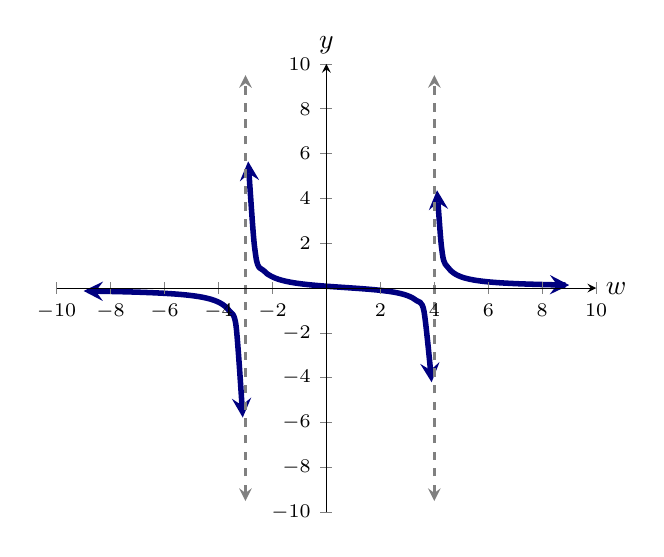
\begin{tikzpicture} 
  \begin{axis}[
            domain=-10:10, ymax=10, xmax=10, ymin=-10, xmin=-10,
            axis lines =center, xlabel=$w$, ylabel=$y$,
            ytick={-10,-8,-6,-4,-2,2,4,6,8,10},
            xtick={-10,-8,-6,-4,-2,2,4,6,8,10},
            ticklabel style={font=\scriptsize},
            every axis y label/.style={at=(current axis.above origin),anchor=south},
            every axis x label/.style={at=(current axis.right of origin),anchor=west},
            axis on top
          ]
          
          \addplot [line width=2, penColor, smooth, domain=(-9:-3.1),<->] {(x-1)/((x+3)*(x-4))};
          \addplot [line width=2, penColor, smooth, domain=(-2.9:3.9),<->] {(x-1)/((x+3)*(x-4))};
          \addplot [line width=2, penColor, smooth, domain=(4.1:9),<->] {(x-1)/((x+3)*(x-4))};

          \addplot [line width=1, gray, dashed, domain=(-9.5:9.5),<->] ({-3},{x});
          \addplot [line width=1, gray, dashed, domain=(-9.5:9.5),<->] ({4},{x});

           

  \end{axis}
\end{tikzpicture}
\end{image}





The numerator has the factor $w-1$, which has multiplicity $\answer{1}$, odd.  Therefore $H$ has $\answer{1}$ as a root and the graph has $(1,0)$ as its only intercept, the only place where the graph crosses the horizontal $w$-axis.


The denominator has two factors $w+3$ and $w-4$.  Both have \wordChoice{\choice[correct]{odd} \choice {even}}  multiplicity, therefore, the function changes sign over these singularities and the graph jumps to the other end of the vertical asymptotes.


The degree of the denominator is larger than the degree of the numerator, therefore the $w$-axis is a horizontal asymptote.



The end-behavior is



\[       \lim_{w \to -\infty} H(w) = \answer{0}   \, \text{ and } \,    \lim_{w \to \infty} H(w) = \answer{0}               \]





$\blacktriangleright$ \textbf{Vertical Asymptotes} 





The factor $w+3$ corresponds to the vertical asymptote described by $w = -3$.


Near $-3$, on either side of $-3$, the factors $w-1$ and $w-4$ do not change sign. 



\begin{itemize}
\item The value of $w-1$ is near $-4$ (negative), when $w$ is near $-3$.
\item The value of $w-4$ is near $-7$ (negative), when $w$ is near $-3$.
\end{itemize}

Both factors take on negative values when $w$ is near $-3$.  

Near $-3$, the value of the numerator of $H$ is near $(-4)(-7) = 28$, when $w$ is near $-3$.  \\





The factor $w+3$ does change sign, since its multiplicity is odd.

\begin{itemize}
\item On the left side, where $w < -3$, we have $w+3<0$, negative.
\item On the right side, where $w > -3$, we have $w+3>0$, positive.
\end{itemize}


Therefore, on the left side of $-3$, $H(w) = \frac{neg}{neg \, \cdot \, neg} = negative$.  \\

Plus, the denominator is approaching $0$ making the whole fraction get bigger and bigger negatively.

We can see this in the graph.  The graph moves down the left side of the $w=-3$ vertical asymptote.

Since this singularity has an odd multiplicity, we also know that $H$ changes sign across this vertical asymptote.


We can now walk through the sign changes of $H$.

\begin{itemize}
\item $w = 1$ is a zero of $H$ with odd multipicity.  The sign of $H$ changes across this zero. The graph crosses the $w$-axis at the $(1, 0)$ intercept.
\item $w = 4$ has an odd singularity. The sign of $H$ changes across this singularity.  The graph jumps to the other infinity across the vertical asymptote.
\end{itemize}



We can now categorize the singularity behavior for $H$.

\begin{itemize}
\item $\lim\limits_{w \to -3^-} H(w) = -\infty$
\item $\lim\limits_{w \to -3^+} H(w) = \infty$
\item $\lim\limits_{w \to 4^-} H(w) = -\infty$
\item $\lim\limits_{w \to 4^+} H(w) = \infty$
\end{itemize}

$H$ has no global or local maximums or minimums.





\textbf{Range:} \\


On the interval $(-3, 4)$, $H$ is continuous.

\begin{itemize}
\item $\lim\limits_{w \to -3^+} H(w) = \infty$
\item $\lim\limits_{w \to 4^-} H(w) = -\infty$
\end{itemize}

That gives us a range for $H$ of $(-\infty, \infty )$.

\end{example}







\subsection*{Sign Changes}

For rational functions, the sign can change only at a zero of odd multiplicity or a singularity of odd multiplicity. This is helpful when graphing. These requirements can force the graph to go in particular directions.



















\begin{center}
\textbf{\textcolor{green!50!black}{ooooo-=-=-=-ooOoo-=-=-=-ooooo}} \\

more examples can be found by following this link\\ \link[More Examples of Analysis]{https://ximera.osu.edu/csccmathematics/precalculus1/precalculus1/libraryAnalysis1/examples/exampleList}

\end{center}







\end{document}
